The subject of this thesis was essentially born out of joining the science team of 
an up-coming spectropolarimeter and velocimeter 
called \spirou{} (un SpectroPolarim\`{e}tre 
InfraRouge; \cite{thibault12, artigau14}) as a first-year grad student. 
The instrument is a next-generation near-IR 
spectropolarimeter for the \emph{Canada-France-Hawaii Telescope} (CFHT) and is 
scheduled for first-light in early 2018. The proceeding sections describe the 
instrument and its main science objectives but there is no better summary than what 
is shown in Fig.~\ref{fig:spiroucomic}. For the linguistically privileged I suppose. 

\begin{figure}
\centering
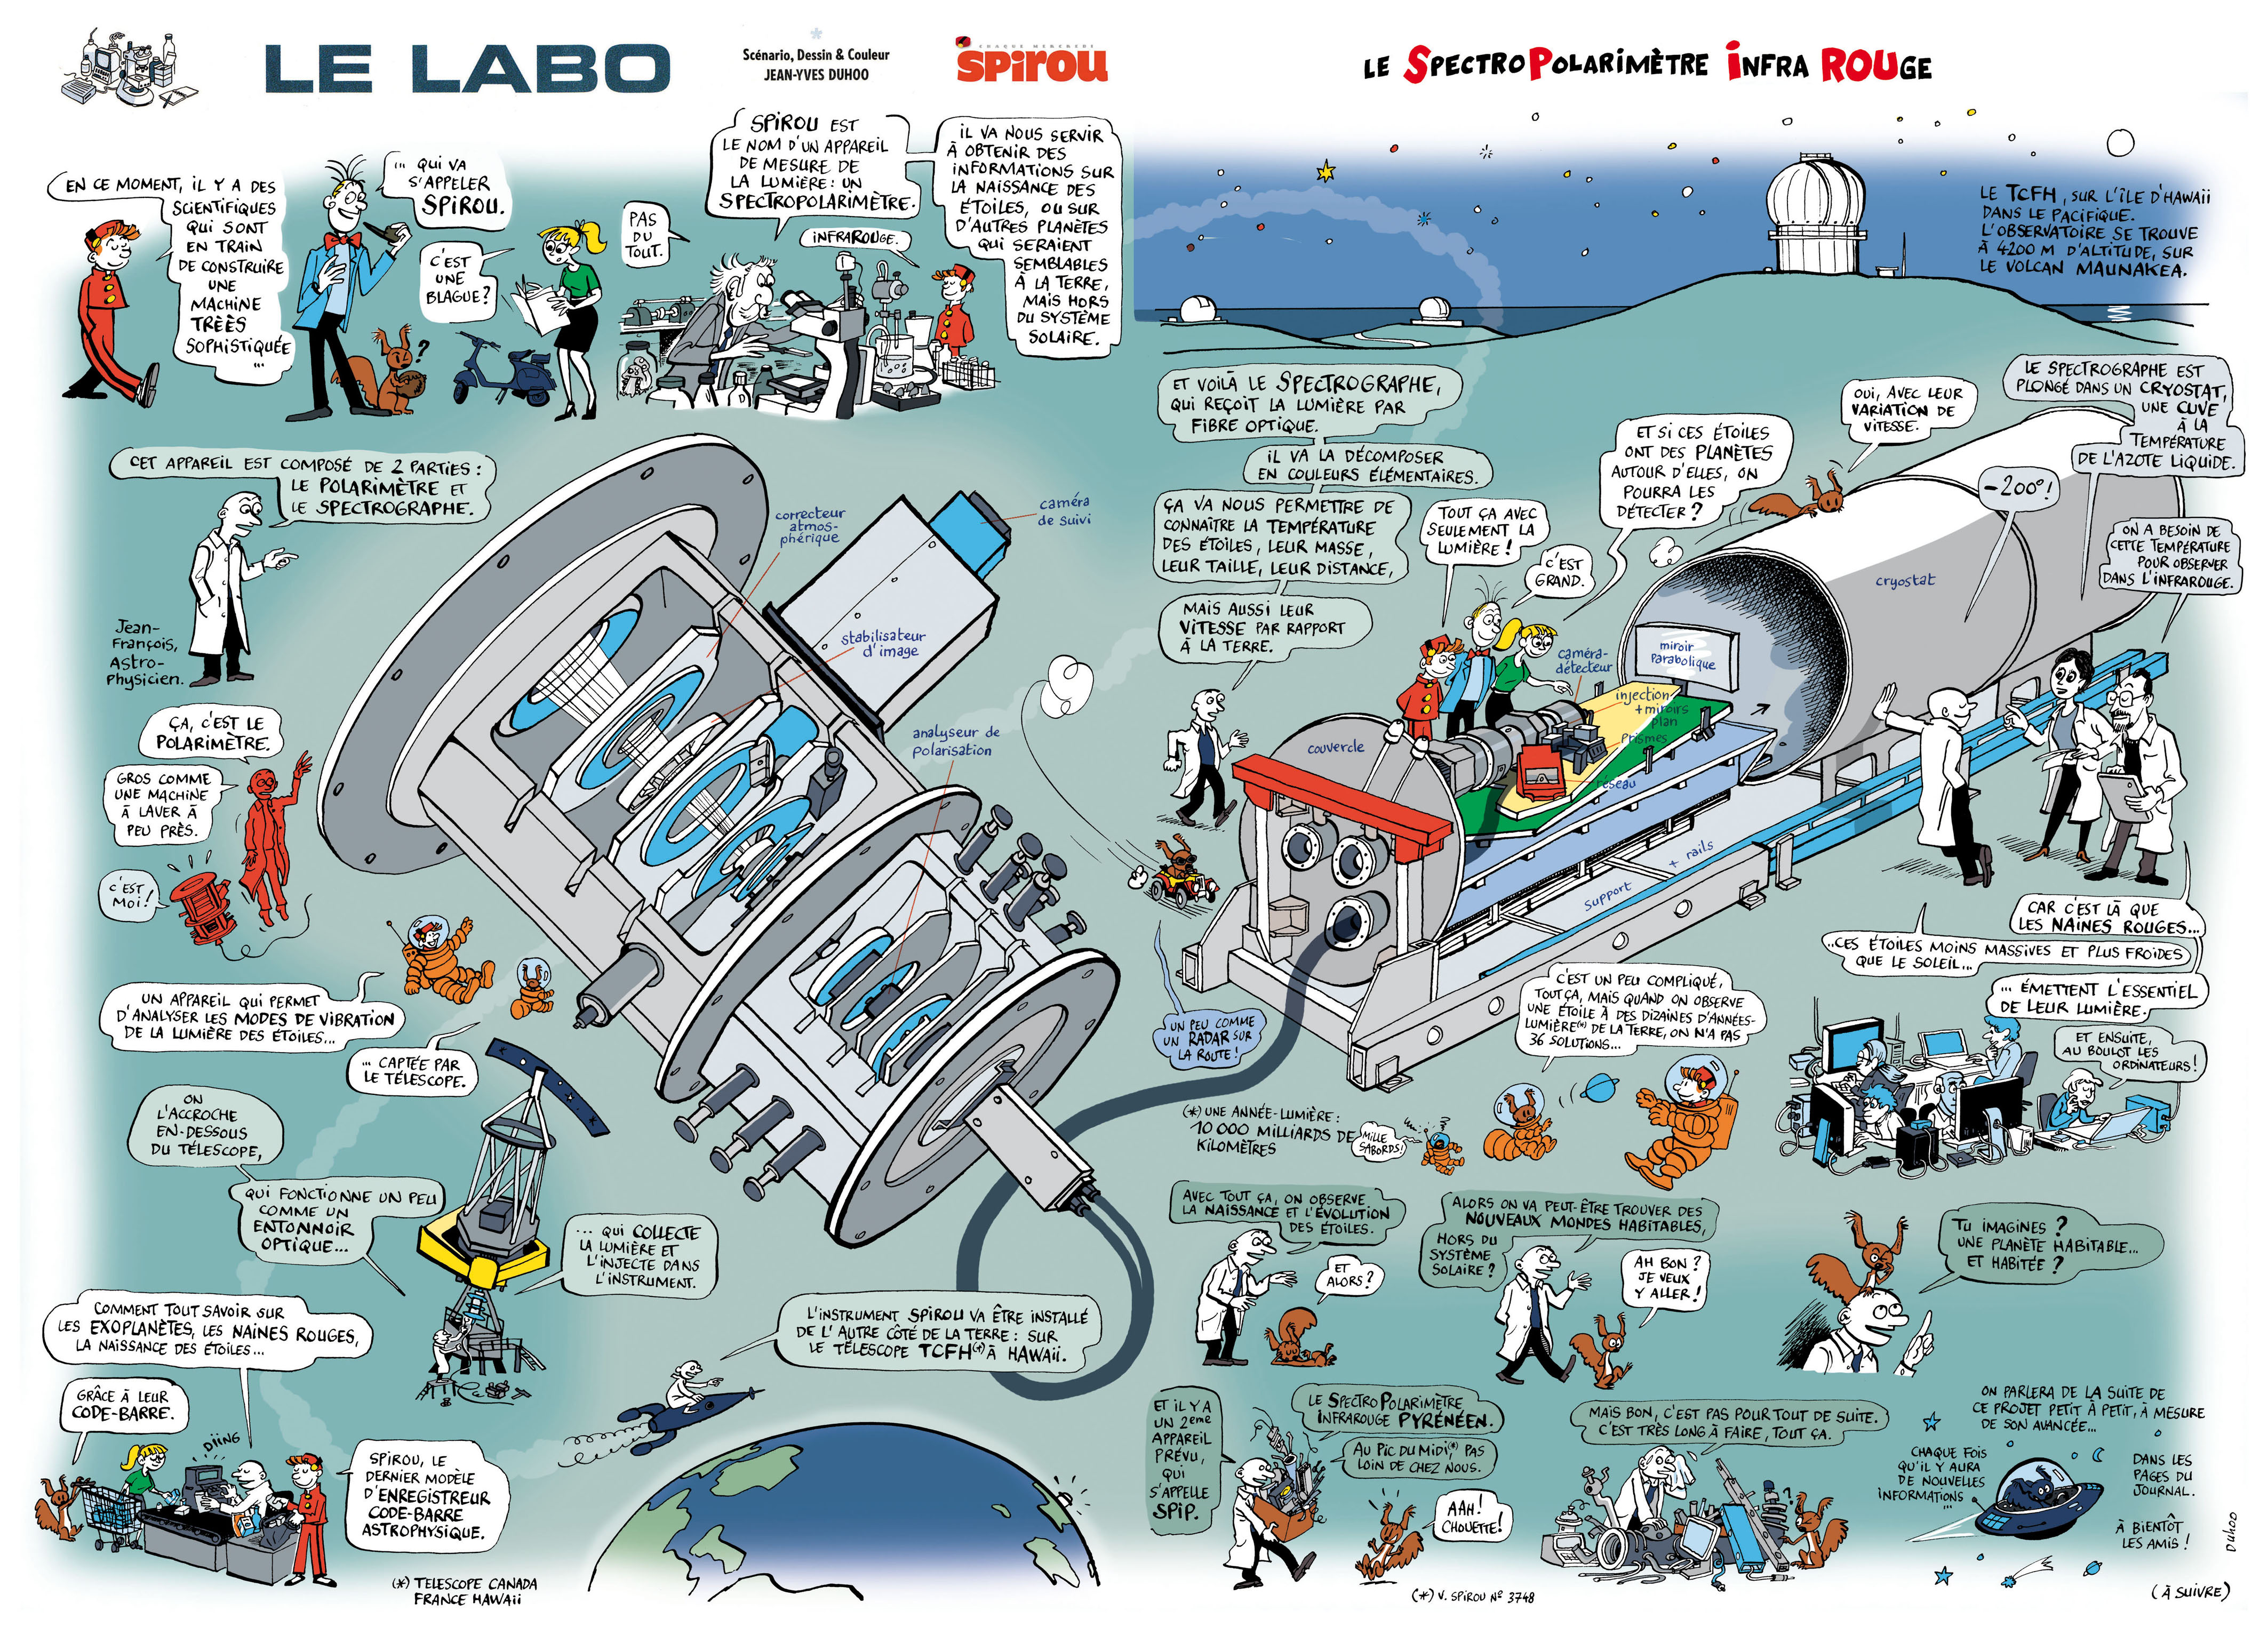
\includegraphics[scale=.4]{figures/SPIROU1-300.jpg}
\caption{SPIRou comic. (Image courtesy of \'{e}ditions Dupuis).
\label{fig:spiroucomic}}
\end{figure}

\section{Instrument Overview} \label{sect:instrument}
Most of the information in this section comes from \cite{donati14a}. \\

As mentioned, \spirou{} is a hi-resolution ($R=\lambda / \Delta \lambda \sim 75$ 
000) near-IR spectropolarimeter. Its simultaneous 
spectral coverage spans the YJHK bands ($\sim 0.98-2.35 \mu$m). K band coverage is 
unique among many up-coming near-IR velocimeters. That is, other prominent 
near-IR spectrographs such as the Habitable zone Planet Finder (\emph{HPF}; 
\cite{halverson14}) and \emph{CARMENES} \parencite{quirrenbach14} 
only go to J and H band respectively. The K band, at $\sim 2.2 \mu$m, offers 
many more photons from cool objects and contains more M-dwarf spectral lines 
than any other near-IR band 
thus significantly contributing to the achievable RV 
precision. At such long wavelengths, the instrument will be permanently installed 
within a cryogenic enclosure to ensure temperature and pressure stability 
with mK stability at 77 K ($\sim -200$ $^{\circ}$C). \\

The spectrograph itself differs from the toy model spectrograph discussed in 
Sect.~\ref{sect:spectrograph}. \spirou{'s} first component is a Cassegrain 
module linking the cryogenic spectrograph to the telescope. This unit contains 
an atmospheric dispersion corrector and wavelength calibration lamps (exact lamps 
TBD). The 
calibration unit is intended to track short and long timescale drifts of the 
observed 
spectra to help ensure a radial velocity stability of 1 \mps{;}  
roughly equivalent to our current `best' optical velocimeters. The second module 
contains the tunable polarimeter (linear or circular polarization) and a fibre 
link for each polarmetric output. The two beams are fed to the spectrograph via the 
fibre link with $>90$\% throughput. The spectrograph itself is double-pass cross 
dispersed and incident on a 4K $\times$ 4K detector. 

\section{Science Cases} \label{sect:spirouscience}
\spirou{'s} two main science goals fall under the categories of exoplanet detection 
and characterization through precision radial velocities and the study of the impact of 
magnetic fields on star and planet formation. In the latter, studies of T-Tauri stars 
requiring the instrument's spectropolarimetric capabilities will also search for 
some of the youngest giant 
exoplanets such as the recent discovery of V830 Tau-b, a hot Jupiter 
around a $\sim 2$ Myr old T-Tauri star \parencite{donati16}. Here we focus 
on the detection and characterization of small planets around M-dwarfs.

\subsection{Why M-dwarfs?} \label{sect:mdwarfs}
First, it is worthwhile to highlight the reasons why M-dwarfs 
are such attractive targets for the detection and characterization of Earth-like
exoplanets. 

\begin{enumerate}
\item \textbf{M-dwarfs are common.} M-dwarfs, with masses of $\sim 0.075-0.6$ 
M$_{\odot}$, are the most common stars in the Milky Way galaxy 
\parencite{chabrier03} and in the solar neighbourhood \parencite{henry09}. This 
enables observers to conduct a statistically significant survey of exoplanets 
around nearby M-dwarfs. Unlike transit surveys which use photometry, 
proximity to Earth is crucial for radial velocity searches as high signal-to-noise 
spectroscopic observations require much larger stellar fluxes ($J \lesssim 10$).
\item \textbf{M-dwarfs host lots of small planets.} The 
planet occurrence rates derived from the sample of Kepler planets 
revealed that small planets ($r_p \leq 4$ R$_{\oplus}$) are common around 
M-dwarfs \parencite{dressing15a, gaidos16}. In fact, the total occurrence rate 
of such planets with orbital periods $< 200$ days was calculated to be 
$\sim 2.5$ planets per M-dwarf. This is in rough agreement with results from 
radial velocity surveys \parencite[e.g.][]{bonfils13} assuming a reasonable 
planetary mass-radius relation. \cite{berta13} argued 
through empirical evidence that this occurrence rate is nearly 
identical for both early and late-type M-dwarfs although the Kepler sample of 
small stars only 
contained late K and early M-dwarfs. This also implies that M-dwarf systems with at least 
one detected planet \parencite[e.g. GJ 1132b;][]{berta15} are likely to contain additional 
planets!

Although the planet occurrence rate around mid-to-late M-dwarfs is largely unconstrained 
at present, the \emph{TRAPPIST} telescope \parencite{gillon11} recently\footnote{In 2015.} 
conducted a pilot transit survey of 50 nearby ultracool dwarfs and discovered a planetary 
system with three transiting planets all with $r_p < 1.17$ R$_{\oplus}$ and on orbits $< 20$ 
days \parencite{gillon16}. The discovery from such a small sample of stars suggests that 
small planets are similarly common around late M-dwarfs as they're known to be around 
early M-dwarfs. 
\item \textbf{Observational signatures of planets around M-dwarfs are large.} 
For a given planet size and mass, both the 
transit depth and radial velocity semi-amplitude are larger for M-dwarfs 
compared to earlier type stars because M-dwarfs represent the class of the 
smallest and lowest mass dwarf stars. Quantitatively, the transit depth is 
$\propto R_s^{-2}$ while the radial velocity semi-amplitude is 
$\propto M_s^{-2/3}$ (Eq.~\ref{eq:K2}). Thus it is easier to detect the signal 
from sought-after Earth-like planets than it is around Sun-like stars. 
\item \textbf{M-dwarf habitable zones have low orbital periods.} 
M-dwarf luminosities are always $< 10$\% that of the Sun. This results in 
their habitable zones lying at much smaller orbital distances than around Sun-like 
stars because of the reduced insolation received by a planet at a given separation. 
For the earliest M-dwarfs 
($M_s\sim 0.6$ M$_{\odot}$) the habitable zone is within 
$\sim 73-190$ days. For the 
latest M-dwarfs ($M_s\sim 0.075$ M$_{\odot}$), the habitable zone is within just 
$\sim 2-6$ days. This is beneficial because short-period planets are generally 
easier to detect than their 
long-period counterparts due to the lessened observational time commitment and 
relative ease of characterizing the full orbital phase of the planet. 
We are therefore most sensitive to HZ planets around M-dwarfs than around any 
other spectral class of star.
\end{enumerate}

As mentioned above, radial velocity surveys are brightness-limited as they are 
often starved for photons. This has been especially true for M-dwarfs because 
most current hi-resolution velocimeters operate at 
optical wavelengths whereas most M-dwarf flux is emitted in the near-to-mid IR 
depending on its spectral type. Therefore 
\spirou{'s} near-IR wavelength coverage makes it an optimal velocimeter for 
searching for planets around M-dwarfs. Our increased sensitivity to 
M-dwarfs will significantly improve our sample of 
nearby M-dwarf planetary systems and hence drastically increase the sample of known 
rocky exoplanets in the solar neighbourhood. Some of the nearest systems will 
be superlative targets for the first ever direct image of a rocky planet with the 
next generation of extremely large telescopes. 

\subsection{Exoplanet Detection: Legacy Survey} \label{sect:survey}
Regarding the detection of new exoplanetary systems, \spirou{} 
will conduct a 5-year long legacy survey of nearby M-dwarfs in the Northern 
sky. The majority of these planetary systems will not be oriented edge-on 
and are therefore 
non-transiting. It is through such a survey that \spirou{} aspires to find the 
\emph{closest potentially habitable world}, which, from the occurrence rate of 
rocky planets around M-dwarfs, the closest potentially habitable planet will 
be within 3.5 pc (95\% confidence) while the closest transiting potentially 
habitable world will be within 14.6 pc \parencite{dressing15a}. The conclusion of the 
survey will also permit the calculation of the planet occurrence rate around 
the latest dwarf stars and possibly some of the earliest ultracool dwarfs. This 
includes an estimation of the value of $\eta_{\oplus}$; the occurrence 
fraction of habitable zone Earth-like planets per star. 

\subsection{Exoplanet Characterization: \emph{TESS} follow-up}
The wealth of newly discovered 
transiting exoplanet candidates from say, \emph{TESS}, will 
require ground-based follow-up observations to confirm their planetary nature 
and measure their masses. 
Unlike the \emph{Kepler} spacecraft which monitored a small patch of the sky 
thus allowing it to probe deeper in apparent magnitude, 
\emph{TESS} will survey the entire sky and obtain a sample of 
comparatively nearby transiting systems compared to \emph{Kepler}. 
By their proximity, the 
majority of candidate transiting planets discovered by \emph{TESS} will 
therefore be within reach of ground-based velocimeters such as \spirou{,} 
which, as was discussed at the end of 
Sect.~\ref{sect:mdwarfs}, is optimized for the detection 
of planets around M-dwarfs whose flux is maximized at near-to-mid IR 
wavelengths. Fig.~\ref{fig:tessmdwarfs} shows the J band magnitude of the 
the 565 Northern sky ($\delta \geq -20$ degrees) \emph{TESS} M-dwarfs (NTMs) 
with at least one transiting planet candidate from the yield simulations 
of \cite{sullivan15}. 
For reference, there are 33 NTMs with $J \leq 9.5$. These are the most attractive 
targets for \spirou{} follow-up because a 1 \mps{} RV stability can be reasonably 
achieved with 15 minute exposures whereas only a nominal RV stability of 
$\sim 3$ \mps{} will be achievable for M-dwarfs with $9.5 \leq J \leq 11.9$. 
There are 330 such NTMs. \\

\begin{figure}
\centering
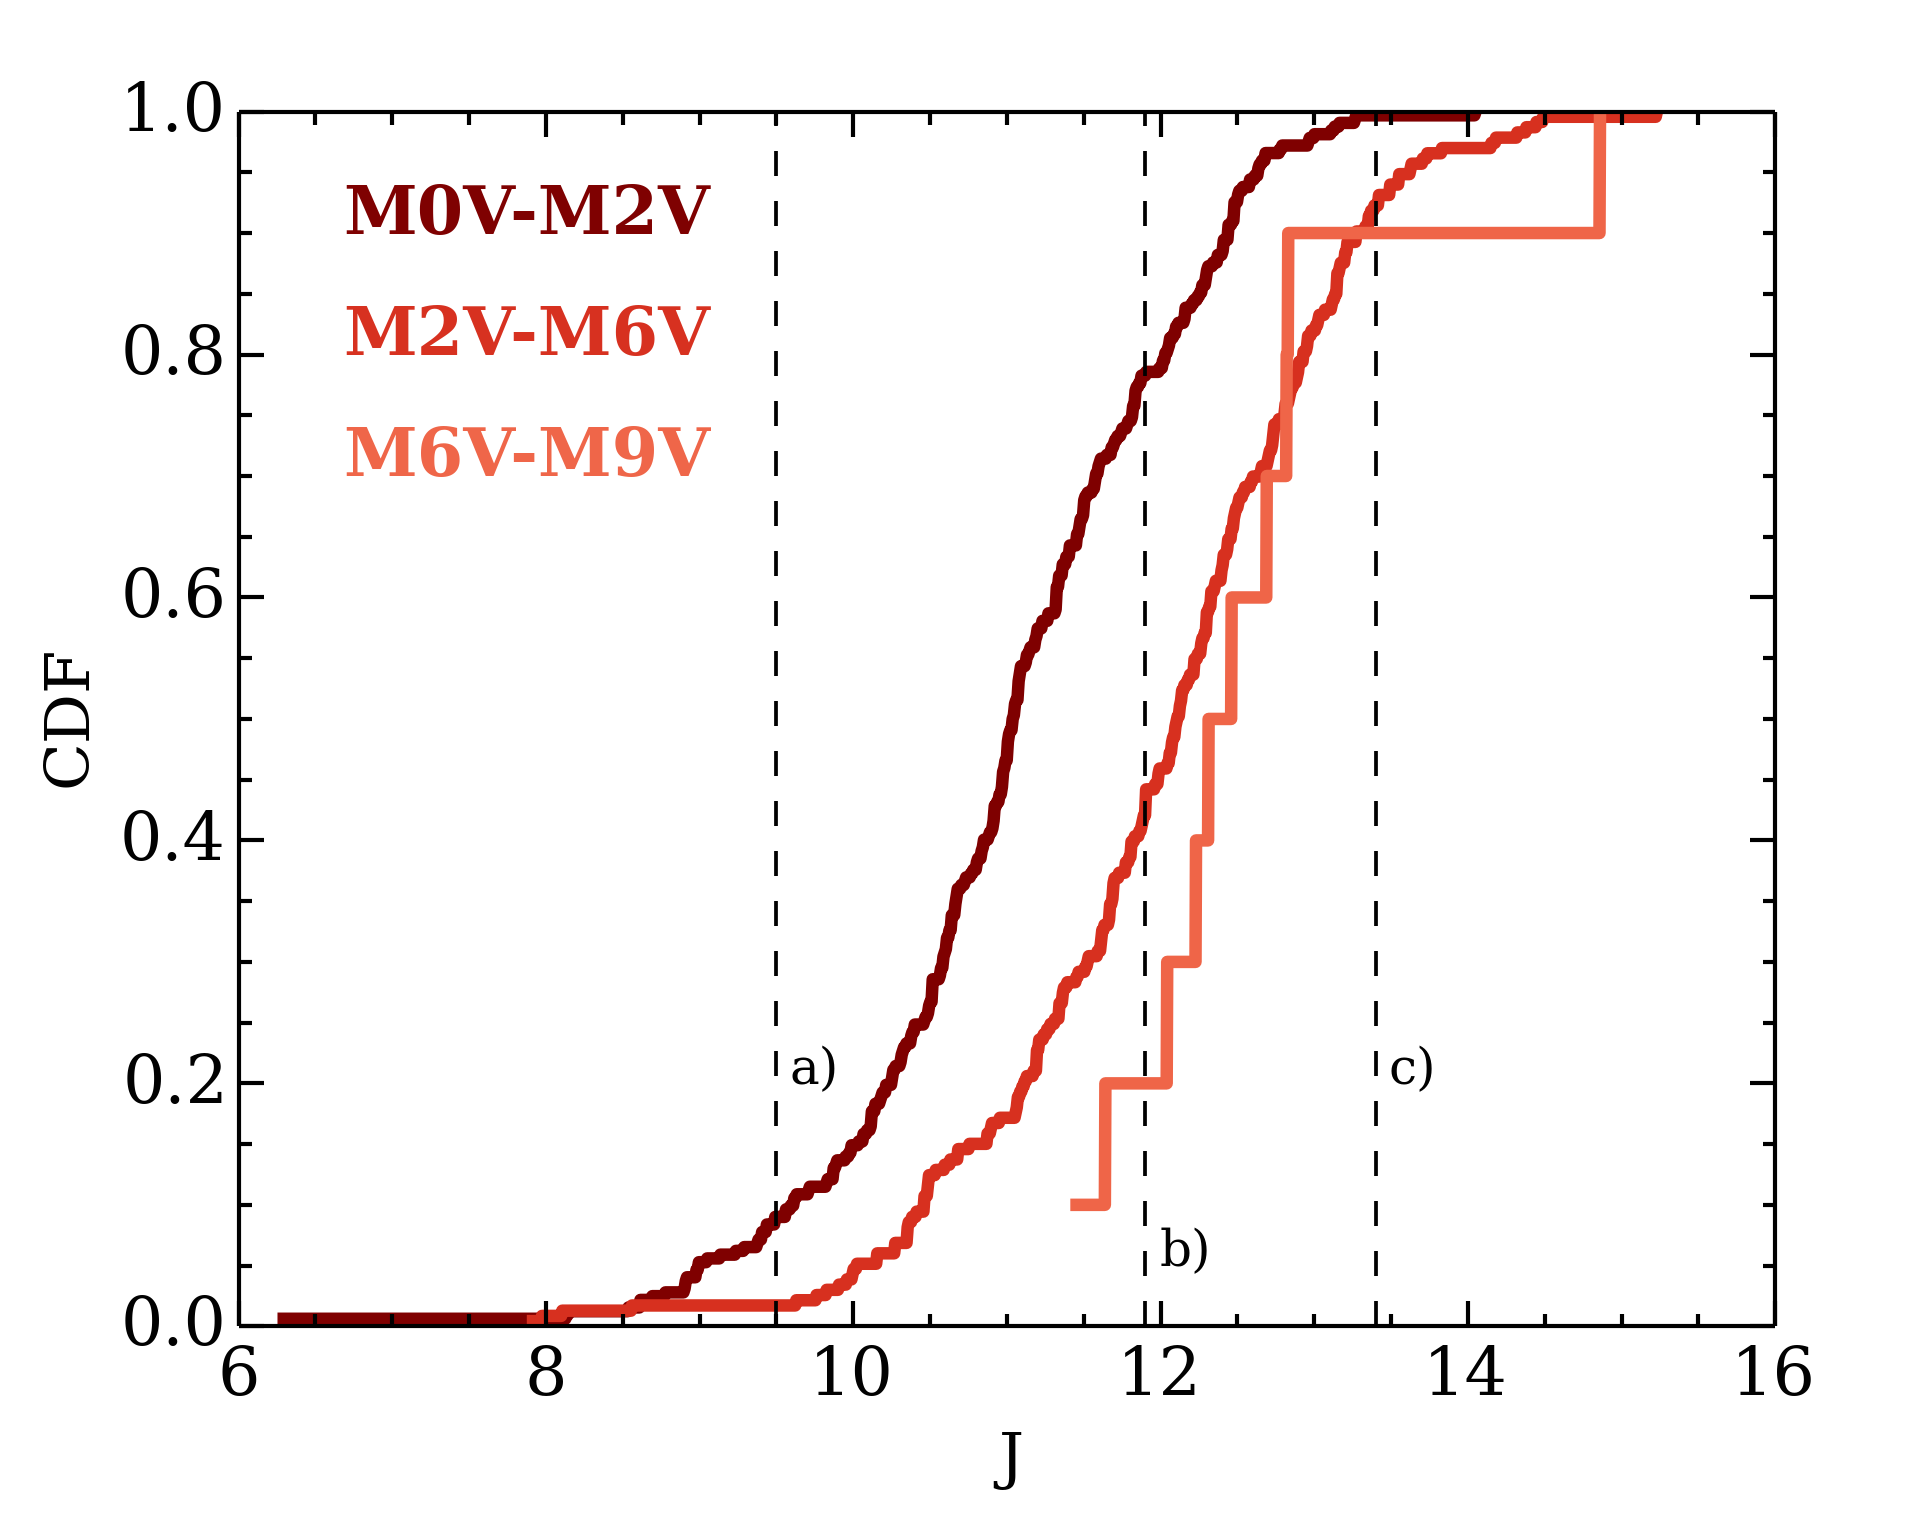
\includegraphics[scale=.5]{figures/tessjmag_sample.png}
\caption{The cumulative distribution function of the Northern sky \emph{TESS} M-dwarfs in 
the (NTMs) in spectral type bins `early', `mid', and `late'. The vertical dashed 
lines depict a) the limiting magnitude for achieving 1 \mps{} stability with $\sim 15$ 
minute exposures,  b) the limiting magnitude for achieving 3 \mps{} stability with 
$\sim 15$ minute exposures, c) the limiting magnitude for achieving 3 \mps{} stability 
with $\sim 60$ minute exposures. \label{fig:tessmdwarfs}}
\end{figure}

Radial velocity follow-up of transiting planets 
is often necessary for confirming the planetary nature of 
\emph{TESS} candidates. Furthermore, the planetary mass is required to infer 
atmospheric properties of transiting planets followed up with transmission 
spectroscopy with \emph{JWST} \parencite{beichman14}. 
One such candidate 
from the K2 mission is K2-18b \parencite{montet15}; a mini-Neptune sized planet 
near the habitable zone of an early M-dwarf. Atmospheric characterization of 
this target is required to distinguish between a `water-world' composition and 
a small solid planet with an extensive gaseous shell. As mentioned, 
modelling of atmospheric 
transmission spectra requires planetary mass measurements in order to constrain the 
planet's pressure scale height via its surface gravity. Radial velocity 
measurements are therefore crucial for i) the study of planetary atmospheres and 
ii) for determining which targets are most conducive to atmospheric 
characterization as observers will preferentially propose to observe targets 
for which the expected signal in transmission is at least at the level of 
detection with the proposed instrumentation.


\iffalse
The upcoming 
\spirou{\footnote{SpectroPolar\'{i}metre InfraRouge.}} 
instrument is a next-generation spectro-polarimeter for the CFHT, operating at 
near-IR wavelengths and will conduct a 3 year survey of nearby M-dwarfs in the 
Northern Hemisphere. A subset of the \spirou{} collaboration are also 
developing a similar near-IR spectrograph 
\emph{NIRPS}\footnote{Near-Infrared Planet Searcher.} to survey the 
Southern sky with contemporaneous polarimetry from \emph{HARPS South} at the 
same site; La Silla Observatory, Chile. It is worth highlighting that 
in addition to forming a large sample of nearby planets orbiting 
M-dwarfs, the joint aim of \spirou{} and \emph{NIRPS} is to find the closest, 
potentially habitable rocky planet. 

\section{Mitigating the Effects of Stellar Jitter with Gaussian processes} 
\label{GP}
Gaussian process regression is a non-parametric method for describing a 
dataset whose measurements are assumed to be correlated over some domain 
(in our case, the time domain). Formally, a Gaussian process (GP) 
is a distribution of random variables which are drawn from 
a $N$-dimensional, multivariate Gaussian distribution, where $N$ is the number 
of data points. For our purposes, a GP noise model is useful for modelling the 
underlying astrophysical noise sources which are known to be present in an 
observed radial velocity timeseries. Such modelling is required to uncover the 
sample of small exoplanets around M-dwarfs whose signal is often comparable 
to the long-term stability of the instrument ($\sim 1$ m/s) and stellar 
jitter can be more than an order of magnitude greater in radial velocity 
for highly active/fast rotating stars.

%Astrophysical contributions to the stellar radial velocity include the 
%presence of (possibly planetary) companions as well as the various effects 
%modulated by the rotation of cold star spots or hot faculae in the 
%stellar photosphere. Spots and faculae have different emissive properties 
%relative to the remaining photosphere due to the large temperature 
%gradient. The ways in which these features contribute to the stellar 
%radial velocity are the following: a rotating, unspotted has both a  
%redshifted and blueshifted limb whose Doppler shifts cancel and remains 
%undetectable. However, if a stellar surface feature is present, it disrupts 
%the homogeneity of the surface can causes a net red or blue shift of 
%incoming photons depending on which limb the feature is occulting. Secondly, 
%the convective nature of M-dwarfs implies that their surfaces are covered in 
%plumes of convective material which result in convective blueshift. The strong 
%magnetic fields associated with star spots and faculae suppress the convective 
%blueshift with the spatial region over which they span, thus causing an 
%additional radial velocity jitter signal. 

In order to disentangle stellar jitter from planetary signals in a radial 
velocity timeseries one requires activity diagnostics in addition to radial 
velocity measurements because planetary signals only manifest themselves in 
the radial velocity signal and not the ancillary timeseries. 
Examples of such diagnostics include photometric measurements, 
the bi-sector inverse slope to the spectral cross-correlation function, and 
the $\log{R'_{HK}}$ activity indicator at visible wavelengths. Because the 
effects of stellar jitter on each on these diagnostics and on the radial 
velocity itself 
are derived from the same physical process in the stellar photosphere, they 
can be modelled as the linear combination of a single underlying GP and an extra
noise term which is unique to each timeseries \citep{rajpaul15}. In practise, 
an ancillary timeseries to the radial velocities (e.g. photometry) is used to 
constrain the GP hyperparameters 
which describe the correlation between data points according to some assumed 
functional covariance. The hyperparameter 
posterior distributions derived from the ancillary timeseries can then, in 
the form of GP hyperparameter priors, be 
applied to radial velocity model containing a GP + Keplarian signal(s) 
\citep{hayword14, grunblatt15}. The 
use of a GP facilitates an increase in accuracy of recovered 
planetary parameters including orbital period, semiamplitude (thus planet 
mass), and orbital eccentricity. 

In order to model the stochastic processes resulting from stellar jitter with 
GP regression, one must parameterize the covariance between data points taken 
at times $t_i$ for $i= 1, \dots, N$ in order to construct the $N \times N$ 
covariance matrix 

\begin{equation}
K_{i,j} = k(t_i, t_j) + \sigma_i^2 \delta_{i,j},
\end{equation}

\noindent where $k(t_i,t_j)$ is the assumed covariance function describing 
the correlation between data points, $\sigma_i$ is the uncertainty on the 
$i^{\mathrm{th}}$ measurement, and $\delta_{i,j}$ is the Kronecker delta. 

For our case in which stellar jitter arises from the rotation of star spots, 
and following similar efforts aimed at measuring stellar rotation periods 
\citep[e.g.][]{mancini15, vanderburg15}, we adopt a quasi-periodic covariance 
function of the form 

\begin{equation}
k(t_i, t_j) = a^2 \mathrm{exp} \left[-\frac{|t_i-t_j|^2}{2\lambda^2} 
-\Gamma^2 \mathrm{sin}^2 \left( \frac{\pi|t_i-t_j|}{P_{\mathrm{rot}}} \right) 
\right],
\end{equation}

\noindent which is parameterized by four hyperparameters: the amplitude of 
the correlations $a$, the exponential decay timescale $\lambda$, the `scale' of 
the correlations $\Gamma$, and the timescale of the periodic term 
$P_{\mathrm{rot}}$ which is interpreted as the stellar rotation period. 
Use of a quasi-periodic (QP) 
GP in modelling the stellar variability associated with rotating 
star spots is favourable because the complicated physics that governs the 
evolution of star spots (i.e. their sizes and lifetimes) need not be strictly 
periodic or sinusoidal. Furthermore, adopting a GP over commonly used 
parametric models of stellar activity allows one to mitigate the degeneracies 
known to be present among parametric stellar jitter model parameters.

The GP hyperparameters are optimized by maximizing the likelihood function 

\begin{equation}
\ln{\mathcal{L}} = -\frac{1}{2} \left( \textbf{y}^T K^{-1} \textbf{y} + 
\ln{\mathrm{det}K} + N \ln{2\pi} \right), \label{like}
\end{equation} 

\noindent where $\mathbf{y}$ is the vector of $N$ measurements. In the case 
of fitting the radial velocities, the model includes a QP GP plus $n$ 
keplarians where $n$ is the assumed number of planets in the system. The vector 
$\mathbf{y}$ is then the residual vector equal to the difference between the 
observed values and the Keplarian model(s). In this way, we optimize the GP 
hyperparameters (which are often well-constrained by their priors) as well as 
the Keplarian orbital parameters. Using the 
method of Markov Chain Monte-Carlo, the model parameter marginalized  
posterior distributions are 
calculated up to a constant using Eq.~\ref{like} and appropriate prior 
probabilities on each parameter. 

Part of the power of GP regression with optimized hyperparameters is 
its predictive power. From a set of measurements \textbf{$y$}, with 
uncertainties \textbf{$\sigma$}, taken at times \textbf{$t$}, the GP process 
is trained, thus leading to the mean predictive distribution at future 
epochs \textbf{$t_*$}:

\begin{equation}
\bar{f}(\mathbf{t_*}) = k(\mathbf{t_*}, \mathbf{t}) [k(\mathbf{t}, \mathbf{t}) 
+ \sigma^2 I]^{-1} \mathbf{y}. 
\end{equation}

\noindent The covariance can then be written as 

\begin{equation}
\mathrm{cov}(f) = k(\mathbf{t_*}, \mathbf{t_*}) - k(\mathbf{t_*}, \mathbf{t}) 
\bar{f} k(\mathbf{t}, \mathbf{t_*}) 
\end{equation}

\noindent where $I$ is the $N \times N$ identity matrix. The predictive power 
of the GP allows one to predict the stellar jitter even in cases for which 
your activity diagnostics are not taken simultaneously with radial velocity 
observations. With that said, given the uncertainties of the GP predictive 
mean, it is desirable to obtain contemporaneous radial velocity measurements 
and activity diagnostics which can be used to model the radial velocity stellar 
jitter at epochs corresponding to your planet hunting measurements.

\section{Planet detection with \spirou{}}
Exoplanet detection via transit and radial velocity observations are highly 
complimentary. For the subset of planets which are 
transiting\footnote{probability $\sim (R_s+r_p)/a \approx 1$\% for an 
Earth-twin in the habitable zone of a typical M-dwarf}, if one assumes a 
stellar radius then planetary radii can be measured along 
with the inclination of the planet's orbital plane. 
Constraints on the orbital inclination coupled with a planet detection in 
radial velocity is used to compute an 
absolute planet mass which, along with the planetary radius, constrains 
the planet's bulk density and surface gravity. Despite only 
about 1\% of planets having orbital geometries conducive to a transit event, 
transit searches have been hugely successful and yielded thousands of 
exoplanet detections with dedicated ground and 
space-based instruments (e.g. \emph{MEarth} \citealt{irwin15}, \emph{Kepler}, 
\& \emph{CoRoT}). The photometric observations themselves are also 
inexpensive to conduct compared to the high-resolution spectroscopic 
observations required by radial velocity measurements thus making transit 
searches better suited to detecting planets around faint target stars and 
allowing for deep and/or wide-field surveys to be conducted more efficiently 
compared to attempting to obtain a statistically significant number of radial 
velocity measurements for an identical sample. The abundance of well-sampled 
photometric light curves are extremely useful for probing stellar jitter which 
can then be incorporated into radial velocity models thus helping to 
distinguish planetary signals for sources of astrophysical noise associated 
with the star (Sect.~\ref{GP}).

The wealth of transiting exoplanet candidates, from say \emph{TESS}, will 
require ground-based follow-up observations to confirm their planetary nature. 
Unlike the \emph{Kepler} spacecraft, \emph{TESS} will survey the entire sky 
rather than monitor a small patch of the sky which allowed \emph{Kepler} to 
probe deeper in apparent magnitude. The 
majority of candidate transiting planets discovered by \emph{TESS} will 
therefore be within reach of ground-based velocimeters including \spirou{}, 
which, as was discussed at the end of 
Sect.~\ref{mdwarfs}, is optimized for the detection 
of planets around M-dwarfs whose flux is maximized at near-to-mid IR 
wavelengths. Accurate radial velocity modelling of \emph{TESS} candidates is 
further facilitate by the fact that photometric timeseries used to train a GP 
will be available for all targets. Part of my work with \spirou{} will be to 
exploit 
the \emph{TESS} light curves to measure photometric variability for the purpose 
of predicting stellar radial velocity jitter \citep{aigrain12} and measuring 
planet masses. This work is necessary for confirming the planetary nature of 
\emph{TESS} candidates including small ($r_p<2$ R$_{\oplus}$), Earth to 
super-Earth planets, most of which are expected to orbit around M-dwarfs 
\citep{sullivan15}; perfect targets for \spirou{.} 

As an aside, we note that a subset of transiting planets will also represent 
viable targets for atmospheric 
characterization with \emph{JWST}. Accurate modelling of planetary transmission 
spectra are also likely to benefit from the use of GPs to model the stochastic 
stellar processes that can obscure planetary atmospheric transmission 
signatures. One such candidate 
from the K2 mission is K2-18b \citep{montet15}; a mini-Neptune sized planet 
near the habitable zone of an early M-dwarf. Atmospheric characterization of 
this target is required to distinguish between a `water-world' composition and 
a small solid planet with an extensive gaseous shell. Modelling of atmospheric 
transmission spectra require planetary mass measurements to constrain the 
planet's pressure scale height via its surface gravity. Radial velocity 
measurements are therefore crucial for i) studying planetary atmospheres and 
ii) for determining which targets are most conducive to atmospheric 
characterization as observers will preferentially propose to observe targets 
for which the expected signal in transmission is at least at the level of 
detection with current instrumentation.

The second aspect of the \spirou{} exoplanet campaign is to conduct a 
brightness-limited 
legacy survey of M-dwarfs in the Northern sky. In addition to characterizing 
\emph{TESS} candidates, I will also spend time analyzing the incoming legacy 
survey data searching for non-transiting planets. 
It is in these data that \spirou{} aspires to find the 
\emph{closest potentially habitable, rocky world}. %From the occurence rate of 
%rocky planets around M-dwarfs, the closest potentially habitable planet will 
%be within 3.5 pc (95\% confidence) while the closest transiting potentially 
%habitable world will be within 14.6 pc \citep{dressing15a}. 
For finding these small planets with 
$K \sim 1$ m/s and no a-prior knowledge or orbital period (unlike the case for 
\emph{TESS} candidates), accurate probes of the stellar radial velocity jitter 
will be required and will likely not be derived for photometric 
light curves, but instead from simultaneous spectroscopic indicators 
\citep{rajpaul15} or from diagnostics of the stellar magnetic field from 
polarimetry \citep{donati15}. %However, mapping of the former observable to 
%radial velocity jitter is not yet fully understood.
The use of a GP to model the stellar jitter in radial velocity will therefore 
be of critical importance for detecting new exoplanets with \spirou{.} 

\section{Studies of detection completeness}
One question commonly asked when formulating a radial velocity observing 
strategy is what is the number of observations required to recover a planet? 
This can pertain 
to searching for planets in a blind manner or in the case for which the 
periodicity of the planet candidate is known from transit observations and the 
expected RV signal can be estimated by assuming some planetary mass-radius 
relationship. Using Monte-Carlo simulations of small planets and constructing 
synthetic radial velocity timeseries which include planetary signals and 
stellar jitter, one can place limits on the number of observations required to 
recover specific planets or, more generally, calculate the detection 
completeness of small planets around M-dwarfs. 
So far we have conducted this analysis for the high-value 
target star GJ 1132, which is known to host a hot rocky planet \citep{berta15} 
whose atmosphere is potentially characterizable with upcoming instrumentation 
given the star's proximity to the Solar system. This work motivates the 
radial velocity follow-up of this particular system and outlines the effort 
required to detect additional planets in the system given that we expect 
such planets to be present according to the frequency of small planets around 
M-dwarfs \citep{dressing15a}.

The next relevant steps are to conduct a similar analysis for i) more 
high-value targets such as K2-18b, ii) the expected yield of \emph{TESS} 
candidates \citep{sullivan15}, and iii) the expected yield from a blind 
survey of the nearest M-dwarfs in the Northern sky. Planet detection 
completeness limits for each of these subcampaigns are useful for the 
efficient strategizing of observations and for statistical purposes once the 
true samples have been uncovered by \spirou{}.
\fi

\section{Point-form Thesis: SPIRou}
\begin{itemize}
\renewcommand\labelitemi{--}
\item~\ref{sect:instrument} \textbf{Instrument Overview}: \spirou{} is a near-IR 
spectropolarimeter and high precision velocimeter scheduled to go on sky at \emph{CFHT} 
in early 2018. 
\item~\ref{sect:spirouscience} \textbf{Science Cases}: \spirou{} will observe M-dwarfs 
in the Northern sky searching for new exoplanets and characterize transiting exoplanet 
candidates such as those from \emph{TESS}.
\end{itemize}
